\documentclass[10 pt,Helvetica, french]{beamer}
% option compress pour réduire la taille des bars
\mode<presentation>
%[compress,hideallsubsections,width=<0.5cm>]
%\usetheme{Darmstadt}
%\usetheme{Malmoe}
%\usetheme{Warsaw}
%\useoutertheme{split}
%\usecolortheme{whale}

%\usepackage[dark]{beamerthemesidebar}
%\usepackage{beamerthemeshadow}
%\usepackage{beamerthemesplit}
%\usepackage{beamerthemebars}
%\usepackage{beamerthemeclassic}
\newcommand{\spac}{\rule[0mm]{0mm}{2mm}}
\usepackage{pgf,pgfarrows,pgfnodes,pgfautomata,pgfheaps,pgfshade}
\usepackage{amsmath,amssymb}
\usepackage[english]{babel}
\usepackage{epic,eepic,bez123}
\usepackage{ bbold }
\usepackage{ upgreek }
\usepackage{eurosym}
%\usepackage[T1]{fontenc}
%\usepackage[ansinew]{inputenc}
%\usepackage[latin1]{inputenc}
%\usepackage{babel,varioref}

%\usetheme{Luebeck}%(encadrements rectangulaires)
%\usetheme{Madrid}%(pas de plan au-dessus)
%\usetheme{Berkeley}%(colonne à gauche)
%\usetheme{Warsaw}%(plan détaillé en haut, utilise la navigation)
%\usetheme{Dresden}%(encadrements rectangulaires)
%\usetheme{Frankfurt}%(pas de paln détaillé en haut)
%\usetheme{Marburg}%(colonne à droite)
%\usetheme{Berlin}%(encadrements rectangulaires)
%\usetheme{Montpellier}

%\usecolortheme{crane}
%\usecolortheme{seahorse}
%\usecolortheme{green}
%\usecolortheme{beetle}
%\usecolortheme{default}
%\usecolortheme{rose}
%\usecolortheme{Berkeley}(inconnu)

%\useoutertheme{smoothtree}
%\useoutertheme{split}
%\usecolortheme{whale}

\setbeamercovered{transparent}
\newtheorem{defi}{Definition}
\newtheorem{theo}{Theorem}
\newtheorem{prop}{Proposition}
\newtheorem{property}{Property}
\newtheorem{coro}{Corollary}
\newtheorem{propannex}{Proposition}
\newtheorem{objective}{Objective}
\newtheorem{res}{Results}


\setbeamertemplate{footline}[text line]{  }
%\setbeamertemplate{footline}[page number]{ }

\newcounter{countAnnexA}
\setcounter{countAnnexA}{0}
\renewcommand{\propannex}{\addtocounter{countAnnexA}{1}
\noindent \large \textbf{Proposition \thesection.\thecountAnnexA}
\normalsize}

\newcommand{\beginbackup}{
   \newcounter{framenumbervorappendix}
   \setcounter{framenumbervorappendix}{\value{framenumber}}
}
\newcommand{\backupend}{
   \addtocounter{framenumbervorappendix}{-\value{framenumber}}
   \addtocounter{framenumber}{\value{framenumbervorappendix}}
}

%\colorlet{orange}{red!70!yellow}% mes petites couleurs que j'aime bien
%\colorlet{mauve}{blue!70!red} \colorlet{brouge}{red!70!blue}
\addtobeamertemplate{footline}{\insertframenumber/\inserttotalframenumber}


\date[September 2016]{S\'{e}minaire LEDa, Universit\'{e} Paris Dauphine, Septembre 2016}
\title[Trade Costs Black Box]{Beyond the Iceberg Hypothesis: \\Opening the Black Box of Transport Costs}
\author[Daudin et al.]{Guillaume Daudin\\
{\footnotesize Universit\'{e} Paris-Dauphine, PSL \& OFCE }\\ \smallskip
J\'{e}rome H\'{e}ricourt \\
{\footnotesize Universit\'{e} de Lille I \& CEPII }\\  \smallskip
Lise Patureau \\
{\footnotesize  Universit\'{e} Paris-Dauphine, PSL}}


\setcounter{framenumber}{-1}
\begin{document}
\begin{frame}[plain]
\titlepage
\end{frame}


\begin{frame}
\frametitle{Motivation}
\begin{itemize}
\item Trade costs have a central role in international economic analysis \vspace{0.1cm}
\begin{itemize}
\item[-] Declining over the second half of the 20$^{th}$ century (Jacks et al., 2008, Novy, 2013) \vspace{0.1cm}
\item[-] But still significant: Average international trade costs = a 74\% markup over production costs (Anderson \& Van Wincoop, 2004)
\end{itemize}
\item What exactly are ``trade costs''?  \vspace{0.1cm}
\begin{itemize}
\item[-] Transaction costs, policy costs, time costs, and transport costs \textit{per se}
\end{itemize}
\item Transport costs are a sizeable share of international trade costs \vspace{0.1cm}
\begin{itemize}
\item[-]  Amount to $\simeq 30\%$ of international trade costs  $\Leftrightarrow$ A 21\% markup over production costs  \vspace{0.1cm}
%\item[-] Elasticity of trade wrt freight costs = -3 (Behar \& Venables, 2011) \vspace{0.1cm}
\end{itemize}
\item[$\Rightarrow$] If much trade policy barriers have been removed, the transport cost component of trade costs remains sizeable \vspace{0.1cm}
\end{itemize}
\textbf{The paper: On international transport costs}

\end{frame}

\begin{frame}
\frametitle{Motivation (cont')}
\begin{itemize}
\item Standard modeling of trade costs: As an ad-valorem tax-equivalent \vspace{0.1cm}
\begin{itemize}
\item[-] As a constant percentage of the producer price per unit traded \vspace{0.1cm}
\item[$\Leftrightarrow$] Part of the ``iceberg cost'' hypothesis (Samuelson, 1954) \vspace{0.1cm}
\begin{itemize}
\item[-] With $p$ the import price, $\widetilde{p}$ the export price, $q$ the quantity traded and $\tau >1$ the trade cost \vspace{0.1cm}
\footnotesize
$$pq = \tau \widetilde{p}q$$
\normalsize
\end{itemize}
\end{itemize}
\item Yet... A debated question \vspace{0.1cm}
\item Would not trade costs rather exhibit an additive structure ?  \vspace{0.1cm} \vspace{0.1cm}
\begin{itemize}
\item[-] Why would it be more costly to transport from Milan to Paris, a pair of Italian shoes at price \euro 300 than a pair of Italian shoes at price \euro 50? \vspace{0.1cm}
\item[-] Pricing shipping often includes an additive component \vspace{0.1cm}
\begin{itemize}
\item[$\star$] UPS: A \$125 fee charged for a 2 pound package from Oslo to NYC (Irrarazabal et al., 2014) \vspace{0.1cm}
\end{itemize}
\item[-] Some trade policy instruments as well (quota license price)
\footnotesize
$$pq = (t+\widetilde{p})q  $$
\end{itemize}
\end{itemize}
\end{frame}


\begin{frame}
\begin{itemize}
\item The structure (additive vs iceberg) of transport costs is not anecdotal \vspace{0.2cm}
\begin{itemize}
\item[-] Many models rely on the tractability of iceberg costs \vspace{0.1cm}
\item[-] Additive trade costs play an important role in shaping the pattern of trade flows (Alchian \& Allen, 1964) \vspace{0.1cm}
\item[-] Strong normative implications, notably w.r.t. the welfare gains of trade liberalization because they distort relative prices (Sorensen, 2014)\vspace{0.1cm}
\end{itemize}
\item Empiric studies
\begin{itemize}
\item[-] The additive structure of trade costs is supported by recent empirical evidence (Irrarazabal et al. 2015, Hummels \& Skiba, 2004)  \vspace{0.1cm}
\item[-] Contrarian view  Lashkaripour (2016) taking into account the fact that more expensive goods are heavier and hence more expensive to transport. Yet  \vspace{0.1cm}
\begin{itemize}
\item[-] This can only apply to goods that are enumerated by items (60\% of US trade)
\item[-] Reasonable hypothesis for goods from the second industrial revolution like cars, it is dubious in the case of ITC goods which importance has been rising since 1994 (the end point of Lashkaripour (2016))
\end{itemize}
\end{itemize}
\item[$\Rightarrow$] Trade costs are likely to display an additive component, but precisely... by how much? \vspace{0.2cm}
\end{itemize}
\textbf{One objective of the paper is to provide an answer to this question}

\end{frame}


\begin{frame}
\frametitle{Our paper in 3 questions (and 3 answers)}
An empirical decomposition of the structure of transport costs \vspace{0.2cm}
\begin{itemize}
\item[(1)]\textbf{ What is the size of the iceberg and the additive costs?} \vspace{0.1cm}
\item[$\Rightarrow$] Provide a quantitative measure of both, using US imports data \vspace{0.1cm}
\begin{itemize}
%\footnotesize{
\item[-] Iceberg cost: 2.5\% of the export price in air, and 3.2\% in vessel (mean value over 1974-2013) \vspace{0.1cm}
\item[-] Additive cost: 1.8\% and 2.9\% of the export price, in air / vessel  \vspace{0.2cm}
%}
\end{itemize}
\item[(2)] \textbf{ What do we lose by skipping the additive part of transport costs?} \vspace{0.1cm}
\item[$\Rightarrow$] We lose much. With the additive term included:\vspace{0.1cm}
\begin{itemize}
%\footnotesize{
\item[-] The estimated iceberg component is reduced by a factor linked to the importance of additive costs (which is kind of obvious) \vspace{0.1cm}
\item[-] A significantly better ``goodness-of-fit'' \vspace{0.1cm}
%}
\end{itemize}
\end{itemize}
\end{frame}


\begin{frame}
\begin{itemize}
\item[(3)] \textbf{ How have international transport costs evolved over time?} \vspace{0.2cm}
\item[$\Rightarrow$] The importance of excluding composition effects \vspace{0.2cm}
%\begin{itemize}
%\footnotesize{
%\item[-]\textit{Pure} transport costs have fallen since 1985 (not 1974), by $\simeq$ 40\% \vspace{0.2cm}
%}
%\end{itemize}
\item[$\Rightarrow$] The importance of including the additive component \vspace{0.2cm}
\begin{itemize}
%\footnotesize{
\item[-] Composition effect is especially strong for the additive costs \vspace{0.2cm}
\item[-] In the air case, the composition effec was not the same on additive and multiplicative costs
%\end{itemize}
%}
\end{itemize}
\end{itemize}
\end{frame}

\begin{frame}
\frametitle{Plan of the talk}
\begin{itemize}
\item Data Sources  \vspace{0.2cm}
\item Empirical Methodology \vspace{0.2cm}
\item Results \vspace{0.2cm}
\item Conclusion
\end{itemize}
\end{frame}


\begin{frame} [label=slide_data]
\frametitle{Data sources}
\begin{itemize}
\item Our measure of international transport costs: The difference between the export price and the import price \vspace{0.1cm}
\item Database: US Imports of Merchandise database \vspace{0.1cm}
\begin{itemize}
\item[-] The export (fas) price, $\widetilde{p}$: the price for one kg of merchandise at the country export point \vspace{0.1cm}
\item[-] The import (cif) price, $p$: the price for one kg of merchandise at the entry in the US \vspace{0.1cm}
\item[-] Yearly basis, from 1974 to 2013, SITC 5-digit classification level, by transport mode (air or vessel) (Could go up to HS-10 with recent data)\vspace{0.1cm}
\end{itemize}
\item[$\Rightarrow$] Our dependent variable: Based on the ratio $p/\widetilde{p}$ \vspace{0.1cm}
\begin{itemize}
\item[-] The RHS are at the 3-digit classification level  \vspace{0.1cm}
\item[-] Estimation at the 4-digit level on some selected years as robustness \vspace{0.1cm}
\item[-] Approximatively 200 sectors (3 digits), from around 200 countries  \vspace{0.1cm}
\begin{itemize}
\item[$\ast$] Around 600-700 sectors at the 4-digit level
\end{itemize}
\end{itemize}
\end{itemize}
\end{frame}

\begin{frame}
\frametitle{More on our database}
\begin{itemize}
\item Implications (and limitations) \vspace{0.1cm}
\begin{itemize}
\item[-] Only cover international transport costs \vspace{0.1cm}
\item[-] Among transport costs, insurance + handling + quantitative freight costs (e.g. not those related to the time value of goods) \vspace{0.1cm}
%\item[$\Leftrightarrow$] Among the 21\% markup from AVW, $\simeq$ 11\% for freight costs (the remaining 9\% for time costs). But ``rough'' estimate. Precisely?  \vspace{0.1cm}
\end{itemize}
\item A rich database to exploit \vspace{0.1cm}
\begin{itemize}
\item[-] US imports, long time period: Broad view of international trade flows \vspace{0.1cm}
\item[-] A reliable database, already used by Hummels (2007), but on a shorter length of time \vspace{0.1cm}
\item[-] We use both the import and the export prices. That allows the estimate the levels of both the ad-valorem and the additive trade costs ($\neq$ Irrarazabal et al., 2015, that uses one year of Norwegian data)
\end{itemize}
\end{itemize}
\end{frame}

\begin{frame}
\frametitle{Empirical specification (1)}
\textbf{The equation at the root of the estimation}
\begin{itemize}
\item Relate the import price $p$ to the export price $\widetilde{p}$ given both additive (per-kg) costs $t$ and ad-valorem costs $\tau$:
$$p = \tau \widetilde{p} + t, \qquad \text{with}\quad \tau \geq 1,\quad t \geq 0$$
\item For product $k$, from country $i$  \vspace{0.1cm}
\item Rewrite to get:
$$\frac{p_{ik}}{\widetilde{p}_{ik}} -1 = \tau_{ik} -1 +\frac{t_{ik}}{ \widetilde{p}_{ik}}$$
\item[$\Rightarrow$] For each year over 1974-2013 (at the $k=$ 5-digit classification level) \vspace{0.1cm}
\begin{itemize}
\item[-] The equation is also mode (air or vessel)- specific
\end{itemize}
\end{itemize}
\end{frame}

\begin{frame}
\frametitle{Empirical specification (2)}
\textbf{The estimation strategy}
\begin{itemize}
\item Two assumptions (as in Irrarazabal et al., 2015) \vspace{0.1cm}
\begin{itemize}
\item[-] Both iceberg and additive costs are separable between the origin country $i$ and the product $k$ dimensions \vspace{0.1cm}
\item[-] Separability in a multiplicative manner for ad-valorem costs and additive manner for per-kg costs \vspace{0.1cm}
\item Additional assumption : all products in a 3-digit sector (s) share the same structure of costs \vspace{0.1cm}
\item[$\Leftrightarrow$] Write $t_{ik^s}$ and $\tau_{ik^s}$ as:
\begin{equation}
 \tau_{ik^s} = \tau_{i} \times \tau_{s}, \qquad t_{ik} = t_{i} + t_{s} \label{eq:specifTC}
 \end{equation}
\end{itemize}
\item Given the constraint $\frac{p_{ik}}{\widetilde{p}_{ik}} -1>0$, the error term should be always positive and multiplicative \vspace{0.1cm}
\item[$\Rightarrow$] The equation of interest becomes:
\footnotesize
$$\frac{p_{ik^s}}{\widetilde{p}_{ik^s}}-1 =\left(\tau_{i} \times \tau_{s} -1+\frac{t_{i} + t_{s}}{\widetilde{p}_{ik^s}} \right)\times \exp(\epsilon_{ik^s})$$
\normalsize
\begin{itemize}
\item[-] With $\epsilon_{ik}$ following a normal law centered on 0
\end{itemize}

\end{itemize}
\end{frame}


\begin{frame}
\begin{itemize}
\item Taking logs, we finally estimate the following equation

\begin{equation}
\ln\left(\frac{p_{ik^s}}{\widetilde{p}_{ik^s}}-1 \right)= \ln \left(\tau_{i} \times \tau_{s}+\frac{t_{i} + t_{s}}{\widetilde{p}_{ik^s}}-1 \right) + \epsilon_{ik^s} \label{eq:est_equation}
\end{equation}
\vspace{0.1cm}
\item A non-linear equation (due to the additive costs)  \vspace{0.1cm}
\item[$\Rightarrow$] Estimation using non-linear squares \vspace{0.1cm}
\begin{itemize}
\item[-] At the basis of the method: Approximate the model by a linear one and refine the parameters by successive iterations \vspace{0.1cm}
\item[-] The criterion for convergence: That the sum of the squares of the residuals does not increase from one iteration to the next \vspace{0.1cm}
\item[-] Eliminate potential influence of outliers: Exclude the 5 percent of the upper and lower tails of the distribution 
\end{itemize}
\end{itemize}
\end{frame}


\begin{frame}
\frametitle{Empirical specification (3)}
\textbf{How to characterize the importance of additive costs relatively to iceberg?} \vspace{0.1cm}
\begin{itemize}
\item Estimate Equation (\ref{eq:est_equation}) constraining $t=0$ \vspace{0.1cm}
\item[$\Rightarrow$] Estimate \textit{two} equations, for each year over 1974-2013, by transport mode (air/ocean)\vspace{0.1cm}
\begin{itemize}
\item[-] With additive costs included:
%\footnotesize
\begin{equation}
\ln\left(\frac{p_{ik^s}}{\widetilde{p}_{ik^s}}-1 \right)= \ln \left(\tau_{i} \times \tau_{s}+\frac{t_{i} + t_{s}}{\widetilde{p}_{ik^s}}-1 \right) + \epsilon_{ik^s}
\end{equation}
%\normalsize
\begin{itemize}
\item[$\Rightarrow$] By year and transport mode, $\simeq$ 800 fixed effects to estimate   \vspace{0.1cm}
\end{itemize}
\item[-] With only ad-valorem costs:
%\footnotesize
\begin{equation}
\ln\left(\frac{p_{ik^s}}{\widetilde{p}_{ik^s}}-1 \right)= \ln \left(\tau_{i} \times \tau_{s}-1 \right) + \epsilon^{ice}_{ik^s} \label{eq:model_nlI}
\end{equation}
%\normalsize
\end{itemize}
\end{itemize}
\end{frame}


\begin{frame}
\begin{itemize}
\item After running the estimates, we re-built: \vspace{0.1cm}
\begin{itemize}
\item[-] With additive costs:
$$\widehat{\tau}^{adv}_{is} = \widehat{\tau_{i}} \times \widehat{\tau_{s}}, \qquad \widehat{t}^{add}_{is} = \widehat{t}_{i} + \widehat{t}_{s}$$
\item[-] With only iceberg costs:
$$\widehat{\tau}^{ice}_{is} = \widehat{\tau_{i}} \times \widehat{\tau_{s}}$$
\end{itemize}
\item  Taking the weighted average over the sector-country dimension, we finally get (by year and transport mode): \vspace{0.1cm}
\begin{itemize}
\item[-] When additive costs are included: $\widehat{\tau}^{adv}$, $\widehat{t}^{add}$  \vspace{0.1cm}
\item[-] With only iceberg costs: $\widehat{\tau}^{ice}$
\end{itemize}
\end{itemize}
\end{frame}

\begin{frame}[label=slide_results_summary]
\frametitle{Result 1: Estimating transport costs over time}
For both the ad-valorem and the additive components \vspace{0.1cm}
\begin{itemize}
\item[-] \footnotesize{Average values over 1974-2013, in percent of the export price \hyperlink{app_results_summary}{\beamergotobutton{More}}  } \vspace{0.1cm}
\end{itemize}
\begin{table}[htbp]
  \centering
  \scriptsize{
  %\caption{Transport costs estimates: Summary \label{tab:summary_results}}
  \begin{center}
    \begin{tabular}{l|cc|cc}
      \hline \hline
    %\multicolumn{5}{c}{Mean value over 1974-2013}   \\
    \# digit & \multicolumn{2}{c}{3 digits} & \multicolumn{2}{c}{4 digits} \\ \hline
    Mode  & Vessel & Air & Vessel & Air \\ \hline
    \multicolumn{5}{l}{With only Ad-Valorem Costs ($\widehat{\tau}^{ice}$)}  \\ \hline
    Mean  & \bf{5.8} & \bf{5.1} & 6.0 & 4.9 \\
    Median & 5.1 & 4.2 & 5.2 & 3.7 \\ \hline
    %Std   & 0.032 & 0.042 & 0.036 & 0.045 \\
    %Min. value & 1.003 & 1.001 & 1.003 & 1.000 \\
    %Max. value & 1.304 & 1.685 & 1.408 & 2.051 \\ \hline
    \multicolumn{5}{l}{With Additive \& Ad-Valorem Costs } \\ \hline
   \multicolumn{5}{l}{\textit{Ad-valorem term} ($\widehat{\tau}^{adv}$)}\\ \hline
    Mean  & \bf{3.2} & \bf{2.5} & 3.3 & 2.4 \\
    Median & 2.8 & 1.8 & 2.8 & 1.6 \\ \hline
    %Std   & 0.023 & 0.023 & 0.025 & 0.026 \\
    %Min. value & 1.001 & 1.000 & 1.000 & 1.000 \\
    %Max. value & 1.227 & 1.474 & 1.264 & 1.537 \\ \hline
    \multicolumn{5}{l}{\textit{Additive term }($\widehat{t}^{add}/\widetilde{p}$)} \\ \hline
    Mean  & \bf{2.9} & \bf{1.8} & 2.8 & 1.9 \\
    Median & 1.9 & 0.7 & 1.7 & 0.8 \\ \hline
    %Std   & 0.041 & 0.034 & 0.039 & 0.034 \\
    %Min. value & 0.000 & 0.000 & 0.000 & 0.000 \\
    %Max. value & 2.941 & 13.303 & 3.197 & 11.440 \\ \hline
       \multicolumn{5}{l}{\textit{Data} }\\ \hline
    Mean &5.3 &5.0 & 5.6&3.9 \\
    Median  &4.3 & 2.0 &4.4 & 1.9 \\  \hline
    \# obs. & 29279 & 28207 & 29317 & 27680 \\
    \# origin country & 188 & 191 & 188 & 189 \\
    \# products & 230 & 211 & 666 & 567 \\    \hline \hline
  \end{tabular}
%\parbox[l]{8cm}{\tiny{Notes: Statistics are obtained weighting each observation by its value.}}
%. The additive term is expressed in fraction of fab price. ($^\ast$): Four 4-digit estimation: 0n selected years. ($^{\ast \ast}$): 1989 omitted in 3 digit estimation for air.}}
\end{center}}
  \end{table}%
 \end{frame}

 \begin{frame}
\frametitle{Result 1: Comments}
\begin{itemize}
\item Transport costs are sizeable \vspace{0.1cm}
\begin{itemize}
\item[-] Add $\simeq$ a 5\% margin over the export price \vspace{0.1cm}
\item[-] Lower than the 21\% markup taken from AVW, but  \vspace{0.1cm}
\begin{itemize}
\item[$\ast$] AVW decompose the 21\% markup in 9\% of time costs and 11\% in pure freight costs  \vspace{0.1cm}
\item[$\ast$] Their 11\% markup: A ``rough'' estimate, based on Hummels (2001) with 1994 data \vspace{0.1cm}
\item[$\ast$] Our data are only for the US, which presumably has lower trade costs \vspace{0.1cm}

\end{itemize}
\item[$\Rightarrow$] Our work: A more precise and exhaustive estimation of international transport costs \vspace{0.1cm}
\end{itemize}
\item Opening the black box of transport costs \vspace{0.1cm}
\begin{itemize}
\item[-] Iceberg cost: 2.5\% and 3.2\% of the export price in Air \& Vessel resp.
\item[-] Additive cost: 1.8\% and 2.9\% of the export price \vspace{0.1cm}
\end{itemize}
\item[$\Rightarrow$] Valuable insights for related papers more theoretically-oriented, in need for calibration
\end{itemize}
\end{frame}


\begin{frame}[label=slide_result2]
\frametitle{Result 2: Additive transport costs do matter}
\begin{itemize}
\item International transport costs: A sizeable additive component  \vspace{0.2cm}
\begin{itemize}
\item[-] Omitting the additive term substantially biases the iceberg component upwards (Table 1) (which is kind of obvios) \vspace{0.2cm}
\begin{itemize}
\item[$\ast$] The ad-valorem cost is reduced by a factor of 2 when additive transport costs are included in the estimation  \vspace{0.2cm}
\item[$\ast$] From 5.8\% to 3.2\% in ocean shipping (mean value over the period) \vspace{0.2cm}
\item[$\ast$] From 5.1\% to 2.5\% in Air transport \vspace{0.2cm}
\end{itemize}
\item[-] A sizeable share of the additive component in total transport costs \vspace{0.2cm}
\begin{itemize}
\item[$\ast$] 48.2\% in average for ocean, 42.3\% for air  \vspace{0.2cm}
\item[$\ast$] A result that holds throughout the period \hyperlink{slide_fig1}{\beamergotobutton{See Figure 1}} \vspace{0.1cm}
\end{itemize}
\end{itemize}
\end{itemize}
\end{frame}


\begin{frame}[label=slide_goodnessfit]
\begin{itemize}
\item A better quality of fit with the additive component included \vspace{0.2cm}
\begin{itemize}
\item[-] Compare the goodness-of-fit of Model (\ref{eq:est_equation}) (with additive TC)  \vspace{0.1cm}
\item[ ] vs Model (\ref{eq:model_nlI}) (without additive TC) \vspace{0.1cm}
\item[-] Various measures of goodness of fit \vspace{0.1cm}
\begin{itemize}
\item[$\ast$] The $R^2$ (the larger the value, the better the fit) \vspace{0.1cm}
\item[$\ast$] Standard Error of Regression (SER) (the smaller the value, the better the fit) \vspace{0.1cm}
\item[$\ast$] The Akaike Information Criterion (the lower AIC, the better the fit) \vspace{0.1cm}
\item[$\ast$] The log-likelihood ratio test ($H_0$: both models are equivalent) \vspace{0.1cm}
\end{itemize}
\end{itemize}
\item[$\Rightarrow$] A systematically better goodness of fit when including the additive component  \vspace{0.1cm}

\begin{itemize}
\item[-] \hyperlink{app_goodnessfit}{\beamergotobutton{See the results}} \vspace{0.1cm}
\item[-] Even when taking into account the additional degrees of freedom
\end{itemize}
\end{itemize}
\end{frame}

\begin{frame}[label = slide_fig1]
\frametitle{Result 3: Characterizing the trends of transport costs }
\begin{itemize}
\item Study the shares of both ad-valorem and additive components in total transport costs  \hyperlink{slide_result2}{\beamergotobutton{Go back to Result 2}} \hyperlink{slide_comment_compositioneffects}{\beamergotobutton{Go back to Main findings}}
\begin{figure}[htbp]
%\caption{Decomposing Transport costs (Yearly mean value, 3 digits)}
%\label{fig:decomp_TC_3d}
\begin{center}
\begin{tabular}{cc}
{\scriptsize (a) Air } & {\scriptsize  (b) Vessel}\\
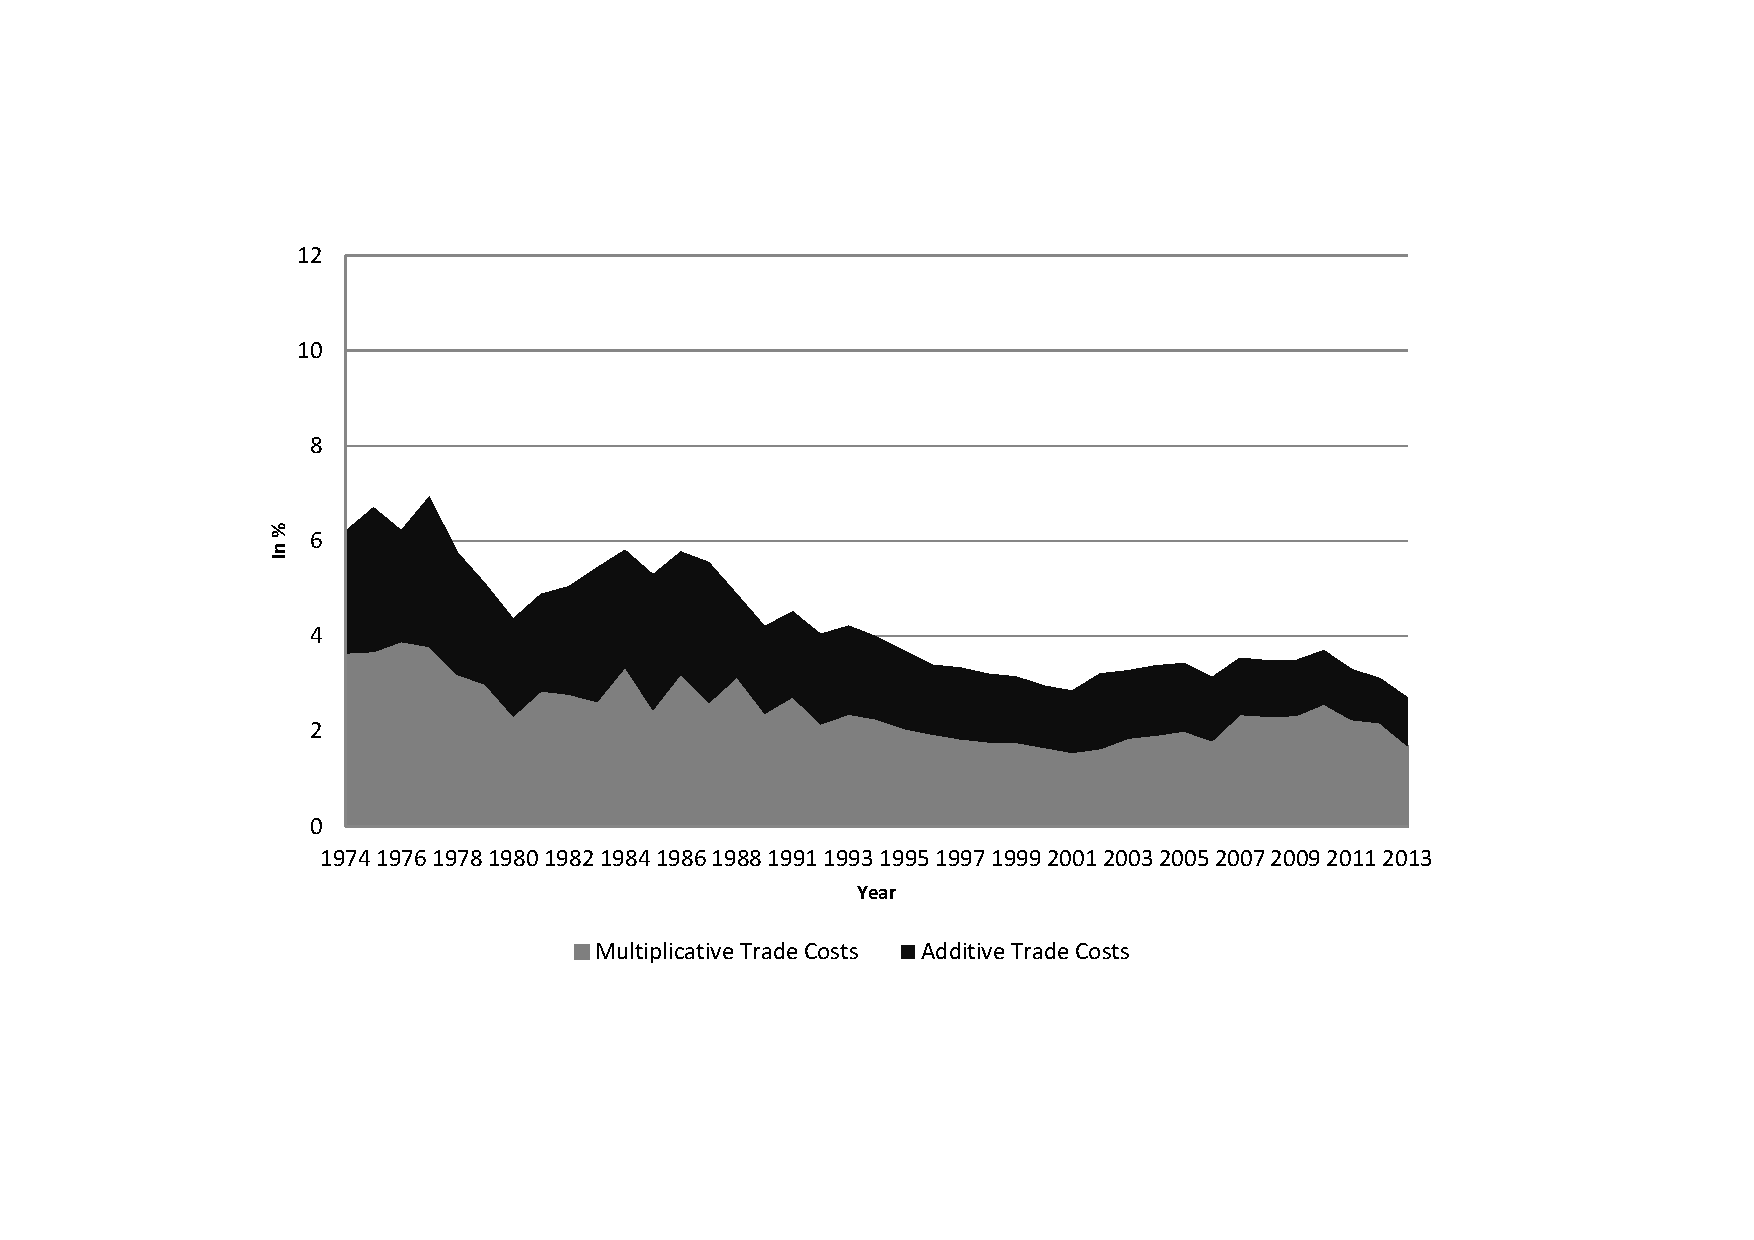
\includegraphics[width=5cm, height=4cm]{Fig2a_decompTC_air_3d.pdf}
& 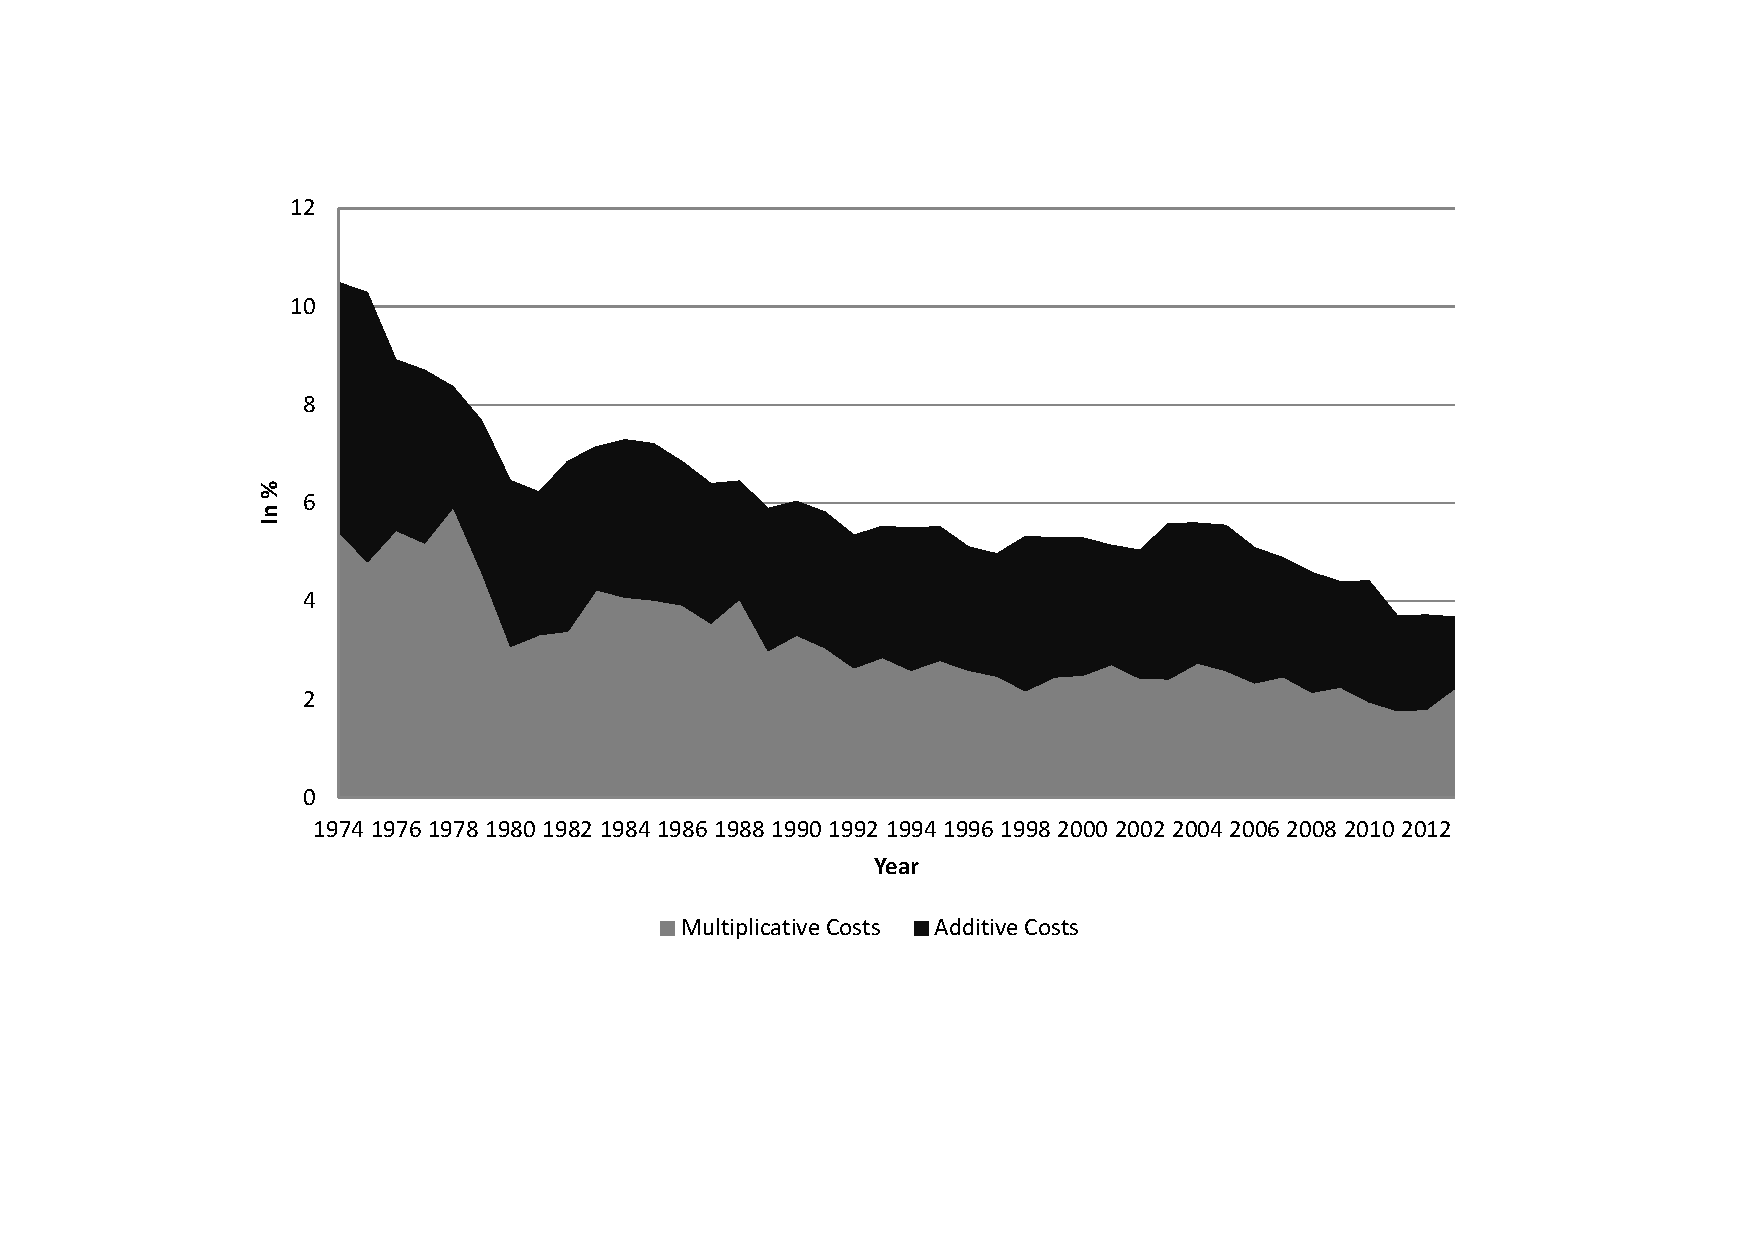
\includegraphics[width=5cm,height=4cm]{Fig2b_decompTC_vessel_3d.pdf} \\
\end{tabular}\end{center}
\end{figure}
\begin{itemize}
\item[-] Lower overall transport costs in Air than in Vessel \vspace{0.1cm}
\item[-] Downward trend for both modes since 1974 \hyperlink{app_fig1}{\beamergotobutton{Robustness of this result}}\vspace{0.1cm}
%\item[-] Slighlty ore pronounced in ocean shipping \vspace{0.1cm}
\begin{itemize}
\item[$\star$] A 50\% decrease in Air, a 60\% decrease in Vessel \vspace{0.1cm}
\end{itemize}
\end{itemize}
\end{itemize}
\end{frame}


\begin{frame}
\frametitle{Time trends in transport costs \& composition effects }
\begin{itemize}
\item Does it mean a decrease in transport costs \textit{per se}? Not necessarily \vspace{0.2cm}
\item The change in overall transport costs over time: \vspace{0.1cm}
\begin{itemize}
\item[-] Depend on the evolution of per product- per partner costs, \vspace{0.1cm}
\item[-] But also on the composition of trade flows \vspace{0.2cm}
\begin{itemize}
\item[$\star$] Over time, import more goods that are cheaper to transport, and/or from countries with which it is cheaper to trade \vspace{0.1cm}
\end{itemize}
\end{itemize}
\item[$\Rightarrow$] Necessary to eliminate the composition effects of trade flows, to isolate the evolution of transport costs \textit{per se}   \vspace{0.1cm}
\item[$\Rightarrow$] What we do, in accordance with Hummels (2007)
\end{itemize}
\end{frame}


\begin{frame}
\frametitle{Excluding the composition effects}
\begin{itemize}
\item For the ad-valorem component, we estimate the following equation:
\footnotesize
\begin{eqnarray}
%\widehat{\tau}_{ikt}&=&\delta\times \exp\left(\sum_{i \neq \text{AFG}}\alpha_i.\mathbb{1}_i\right).\exp\left(\sum_{k\neq \text{011}}\beta_k.\mathbb{1}_k\right).\exp\left(\sum_{t \neq 1974}\gamma_t.\mathbb{1}_t\right) .\exp\left(\epsilon_{ikt}\right) \notag \\
\ln(\widehat{\tau}_{ist})&=&\delta +\underbrace{\sum_{i \neq \text{AFG}}\alpha_i.\mathbb{1}_i }_{\ln(\widetilde{\tau}_i)}+ \underbrace{\sum_{s\neq \text{011}}\beta_s.\mathbb{1}_s }_{\ln(\widetilde{\tau}_s)}+ \underbrace{\sum_{t \neq 1974}\gamma_t.\mathbb{1}_t}_{\text{Time trend}}+\epsilon_{ist} \label{eq:compeffects_mult}
\end{eqnarray}
\normalsize
\begin{itemize}
\item[-] With $\widehat{\tau}_{ist} = \widehat{\tau}^{ice}_{ist}, \widehat{\tau}^{adv}_{ist}$ previously obtained  \vspace{0.1cm}
\end{itemize}
\item For the additive component:
\footnotesize
\begin{eqnarray}
%\widehat{t}_{ikt}&=&\left( \prod_{i \neq \text{ARG}}  \alpha_i.\mathbb{1}_i+\prod_{k}\beta_k.\mathbb{1}_k\right).\exp\left(\sum_{t \neq 1974}\gamma_t.\mathbb{1}_t\right) .\exp\left(\epsilon_{ikt}\right) \notag \\
\ln(\widehat{t}_{ist})&=&\ln\left(\delta +  \underbrace{\sum_{i \neq \text{ARG}}  \alpha_i.\mathbb{1}_i}_{\widetilde{t}_i}+ \underbrace{\sum_{s \neq \text{011}}\beta_s.\mathbb{1}_s}_{\widetilde{t}_s}\right) + \underbrace{\sum_{t \neq 1974}\gamma_t.\mathbb{1}_t}_{\text{Time trend}}+\epsilon_{ist} \label{eq:compeffects_add}
\end{eqnarray}
\normalsize
\item Underlying rationale
\footnotesize
\begin{itemize}
\item[-] Equations (\ref{eq:compeffects_mult}) and (\ref{eq:compeffects_add}): Preserve our specification of the ad-valorem and the additive costs (Equation (\ref{eq:specifTC})) \vspace{0.1cm}
\item[-] Equation (\ref{eq:compeffects_mult}) estimated using OLS, Equation (\ref{eq:compeffects_add}) using non-linear least squares (by transport mode)
    \normalsize
\end{itemize}
\end{itemize}
\end{frame}

\begin{frame}[label = slide_compeffects]
\begin{itemize}
\item Exclude the composition effects of transport costs changes  \hyperlink{app_compeffects}{\beamergotobutton{More details}}\vspace{0.1cm}
\item[$\Leftrightarrow$] Isolate the change in the time dimension  \vspace{0.1cm}
\begin{itemize}
\item[-] From the ad-valorem component estimation (Equation (\ref{eq:compeffects_mult})), build the variable $\Gamma_t$ ($\forall~t > 1974$):
\begin{equation*}
 \Gamma_t= \frac {\bar{\tau}_{1974}.\exp(\gamma_t)-1} {\bar{\tau}_{1974}-1}
\end{equation*}
\begin{itemize}
\item[$\ast$] with $\bar{\tau}_{1974} = \exp(\delta+\sum_i \alpha_i + \sum_k \beta_k$) the mean TC in 1974
\end{itemize}
\item[-] For the additive cost, we build the variable ($\forall~t > 1974$)
$$\Gamma^{add}_t = 100 \exp(\gamma_t)$$
\end{itemize}
\item The $\Gamma^{add}_t$ and $\Gamma_t$ series: Interpretation in percentage changes
\begin{itemize}
\item[] with an initial value of 100 for $t=1974$
\end{itemize}
\end{itemize}

\end{frame}

\begin{frame}
\frametitle{Time trends in transport costs \textit{per se}}
\begin{itemize}
\item Total transport costs (composition effects excluded) over time
\end{itemize}
\begin{figure}[htbp]
%\caption{Decomposing Transport costs (Yearly mean value, 3 digits)}
%\label{fig:decomp_TC_3d}
\begin{center}
\begin{tabular}{cc}
\\
 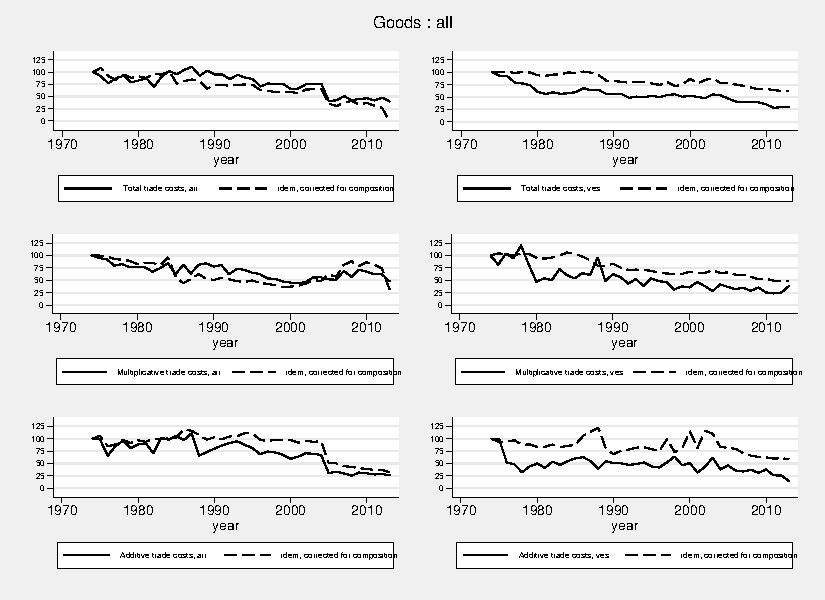
\includegraphics[width=10cm,height=7.5cm]
{graph_composition_all-eps-converted-to.pdf} \\
\end{tabular}
\end{center}
\end{figure}

\end{frame}


\begin{frame}[label=slide_comment_compositioneffects]
\frametitle{What do we find}
\begin{itemize}
\item At the aggregate level  \vspace{0.1cm}
\begin{itemize}
\item[-] Air transport costs were reduced by 50\% and vessel transport costs by 60\%. (as already seen) \vspace{0.1cm}
\item[-] In the case of vessel, a large part of that is a composition effect (reduction in the share of bulky goods because of the relative decline of primary goods) \vspace{0.1cm}
\item[-] The reverse happened for air transport (increase in the shipping of bulky goods) \vspace{0.1cm}
\end{itemize}
\item Additive and multiplicative costs \vspace{0.1cm}
\begin{itemize}
\item[-] The composition effect is especially strong for the additive costs. Maybe bulkiness is more important for additive costs than for multiplicative costs ? \vspace{0.1cm}
\item[-] One might want to think of multiplicative as insurance and additive as shipping of handling. Will that help thinking about the composition effect? \vspace{0.1cm}
\end{itemize}
\end{itemize}
\end{frame}


\begin{frame}
\frametitle{Conclusion: Main findings}
\textbf{Our paper: Empirical evidence about the role of the additive component in international transport costs} \vspace{0.1cm}
\begin{itemize}
\item Provide a quantitative evaluation of both the additive and the ad-valorem components \vspace{0.1cm}
\begin{itemize}
\item[-] Based on the US imports flows from 1974 to 2013 \vspace{0.1cm}
\item[-] Additive cost: amount to 2.8\% of the export price in ocean shipping, 1.8\% in air transport \vspace{0.1cm}
\item[-] Iceberg cost: 3.2\% and 2.5\% for air and ocean respectively \vspace{0.1cm}
\end{itemize}
\item The importance of taking into account additive transport costs \vspace{0.1cm}
\begin{itemize}
\item[-] Additive costs are far from negligible quantitatively \vspace{0.1cm}
\item[-] A better fit of the model when they are taken into account    \vspace{0.1cm}
\end{itemize}
\item Characterize the evolution of transport costs over time \vspace{0.1cm}
\begin{itemize}
\item[-] Importance of the composition effects \vspace{0.1cm}
\end{itemize}
\end{itemize}

\end{frame}

\begin{frame}
\frametitle{Conclusion : What to do next?}

\textbf{Three main possible extensions}
\begin{itemize}
\item On the empirical side: \vspace{0.1cm}
\begin{itemize}
\item[(1)] Compare the trends in transports costs \textit{between} air and vessel (excluding composition effects) \vspace{0.1cm}
\item[(2)] Go deeper in the structural determinants of transport costs \vspace{0.1cm}
\begin{itemize}
\item[$\star$] Identify the respective roles of handling costs, insurance and freight costs at the root of the import-export prices gap \vspace{0.1cm}
\end{itemize}
\end{itemize}
\item On the theoretical side:
\begin{itemize}
\item[(3)]Use our results to explore the role of additive costs \vspace{0.1cm}
\begin{itemize}
\item[$\star$] In shaping international trade flows (trade theory) \vspace{0.1cm}
\item[$\star$] In affecting the international transmission of business cycles (business cycle theory)
\end{itemize}
\end{itemize}
\end{itemize}
\end{frame}


\beginbackup



\appendix



\begin{frame}[label=app_results_summary]
\frametitle{Decomposing transport costs: Summary \hyperlink{slide_results_summary}{\beamergotobutton{Back to slide}}}
\begin{table}[htbp]
  \centering
  \scriptsize{
  %\caption{Transport costs estimates: Summary \label{tab:summary_results}}
  \begin{center}
    \begin{tabular}{l|cc|cc}
      \hline \hline
    \multicolumn{5}{c}{Mean value over 1974-2013}   \\
    \# digit & \multicolumn{2}{c}{3 digits} & \multicolumn{2}{c}{4 digits ($^\ast$)} \\ \hline
    Mode  & Vessel & Air ($^{\ast \ast}$) & Vessel & Air \\ \hline
    \multicolumn{5}{l}{With only Ad-Valorem Trade Costs }  \\ \hline
    Mean  & 1.058 & 1.051 & 1.060 & 1.049 \\
    Median & 1.051 & 1.042 & 1.052 & 1.037 \\
    Std   & 0.032 & 0.042 & 0.036 & 0.045 \\
    Min. value & 1.003 & 1.001 & 1.003 & 1.000 \\
    Max. value & 1.304 & 1.685 & 1.408 & 2.051 \\ \hline
    \multicolumn{5}{l}{With Additive \& Ad-Valorem Trade Costs } \\ \hline
   \textit{Ad-valorem term} & & & & \\ \hline
    Mean  & 1.032 & 1.025 & 1.033 & 1.024 \\
    Median & 1.028 & 1.018 & 1.028 & 1.016 \\
    Std   & 0.023 & 0.023 & 0.025 & 0.026 \\
    Min. value & 1.001 & 1.000 & 1.000 & 1.000 \\
    Max. value & 1.227 & 1.474 & 1.264 & 1.537 \\ \hline
    \textit{Additive term }& & & &   \\ \hline
    Mean  & 0.029 & 0.018 & 0.028 & 0.019 \\
    Median & 0.019 & 0.007 & 0.017 & 0.008 \\
    Std   & 0.041 & 0.034 & 0.039 & 0.034 \\
    Min. value & 0.000 & 0.000 & 0.000 & 0.000 \\
    Max. value & 2.941 & 13.303 & 3.197 & 11.440 \\ \hline
        \# obs. & 29279 & 28207 & 29317 & 27680 \\
    \# origin country & 188 & 191 & 188 & 189 \\
    \# products & 230 & 211 & 666 & 567 \\  \hline \hline
  \end{tabular}
    \end{center}}
\parbox[l]{8cm}{\tiny{Notes: Statistics are obtained weighting each observation by its value. The additive term is expressed in fraction of fab price. ($^\ast$): Four 4-digit estimation: 0n selected years. ($^{\ast \ast}$): 1989 omitted in 3 digit estimation for air.}}
\end{table}%
\end{frame}


\begin{frame}[label=app_fig1]
\frametitle{Ad-valorem costs over time \hyperlink{slide_fig1}{\beamergotobutton{Back to slide}}}
\begin{figure}[htbp]
\caption{Ad-valorem Costs (Yearly mean value, 3 digits)}
\label{fig:mult_alone_withadd}
\begin{center}
\begin{tabular}{cc}
{\small (a) Air } & {\small (b) Vessel}\\
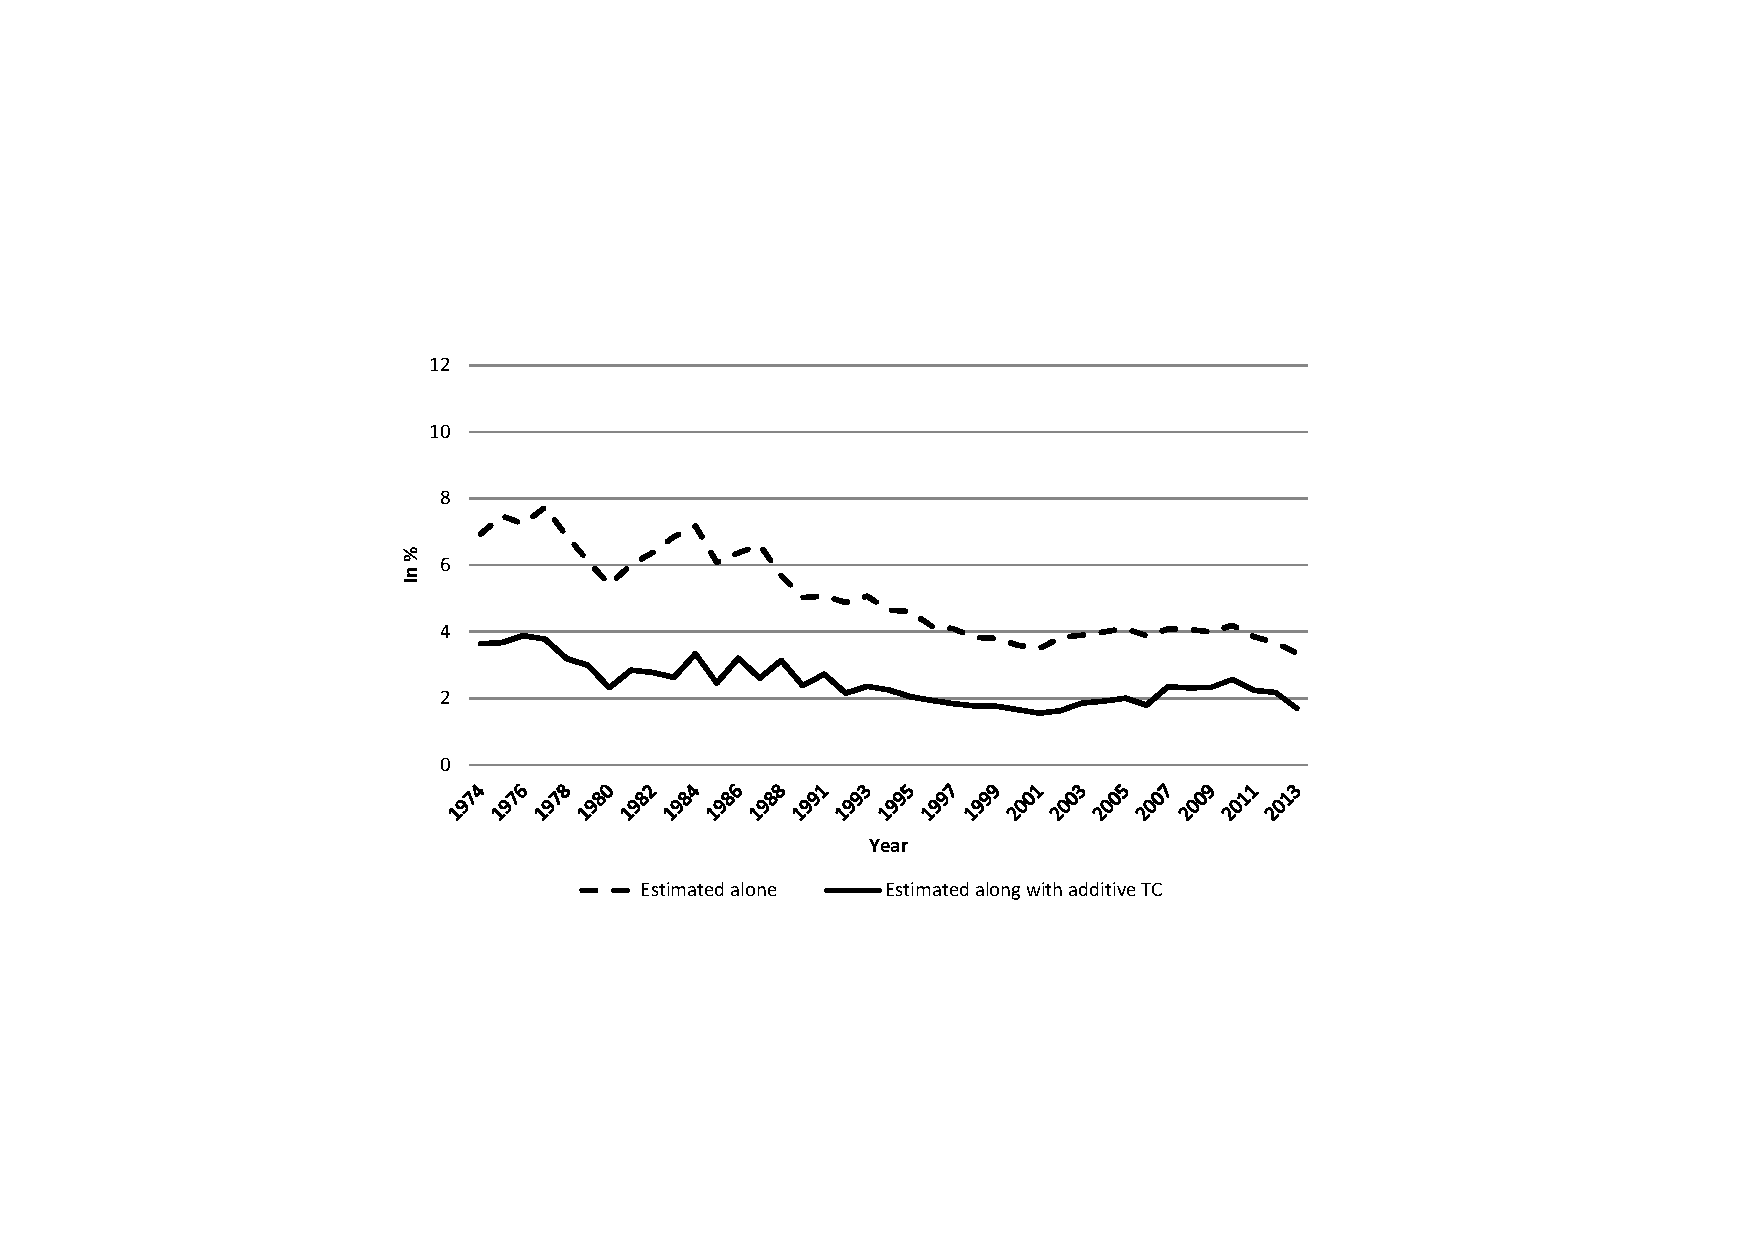
\includegraphics[width=5cm, height=2.5in]{Fig1a_mult_air_3d.pdf}
& 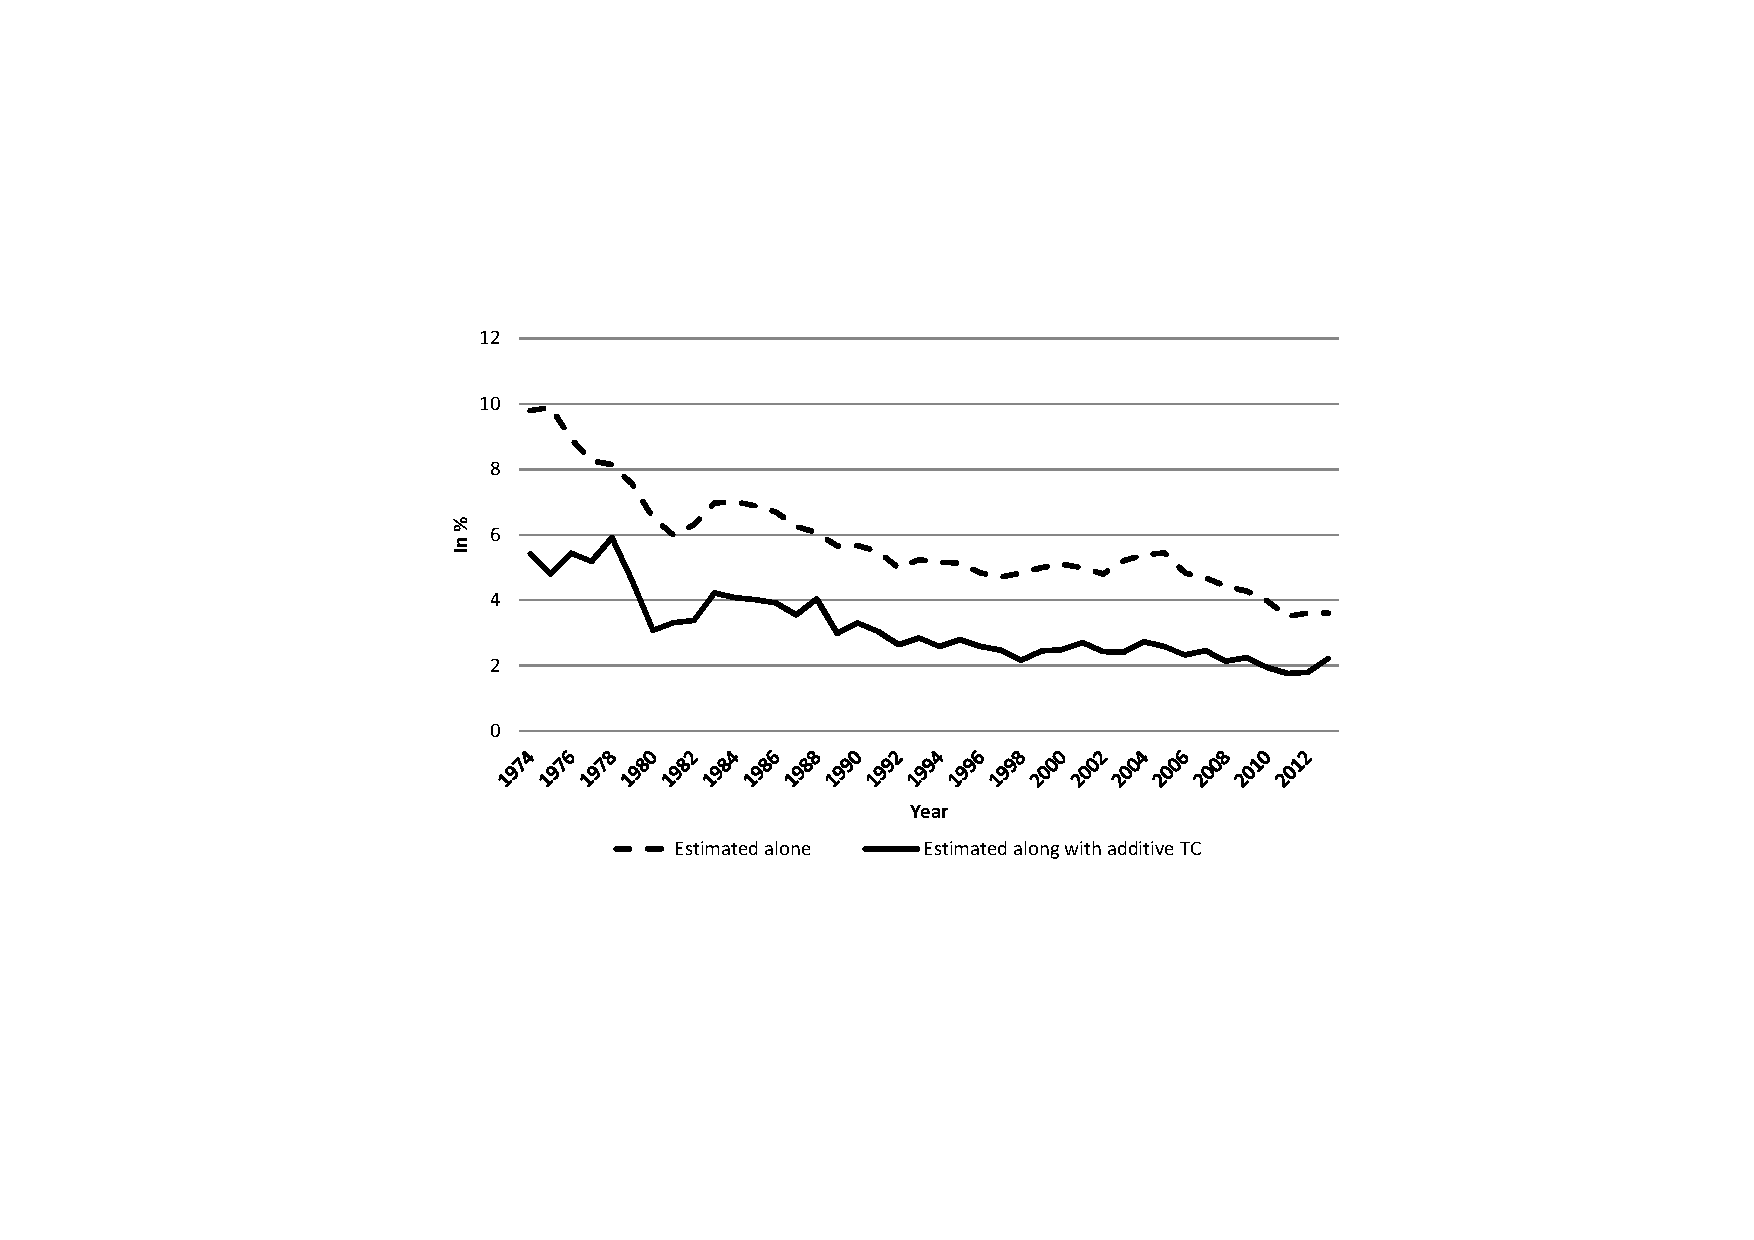
\includegraphics[width=5cm,height=2.5in]{Fig1b_mult_vessel_3d.pdf} \\
\end{tabular}
\end{center}
\end{figure}

\end{frame}



\begin{frame}[label=app_goodnessfit]
\frametitle{More on Result 2: Goodness of fit comparison}
\begin{itemize}
\item Air, 3 digit - level, selected years
\end{itemize}
\begin{table}[htbp]
  \centering
 % \caption{Air: Measures of Goodness-of-fit (3 digits)}
  \scriptsize{
\begin{center}
    \begin{tabular}{l|ccccc|c}
    \hline \hline
    Year  &1980  & 1990  & 2000  & 2010 & 2013 & Mean stat \\ \hline
    \multicolumn{7}{l}{\bf{$R^2$} }\\ \hline
    Term I only &  0.27  & 0.25  & 0.32  & 0.42 & 0.34 & 0.31 \\
    Terms A \& I &  0.65  & 0.63  & 0.64  & 0.51 & 0.46 & 0.60 \\ \hline
    \multicolumn{7}{l}{\textbf{SER}  }  \\ \hline
    Term I only &  0.86  & 0.81  & 0.84  & 0.86 & 0.92 & 0.85 \\
    Terms A \& I &  0.71  & 0.67  & 0.70  & 0.79 & 0.85 & 0.73 \\ \hline
   \multicolumn{7}{l}{\textbf{AIC criteria}}  \\ \hline
    Term I only &  41171.0 & 60715.6 & 87492.6 & 102297.6 & 88191.9 & 70498.1 \\
    Terms A \& I & 35738.4 & 52098.9 & 74954.9 & 95887.1 & 80873.7 & 62285.0 \\ \hline
    \multicolumn{7}{l}{\textbf{Log-likelihood}} \\ \hline
    Term I only &  -20253.5 & -29977.8 & -43341.3 & -50746.8 & -43692.9 & -34888.6 \\
    Terms A \& I &  -17263.2 & -25393.5 & -36788.4 & -47277.5 & -39751.9 & -30508.3 \\
    LL ratio &  5980.6 & 9168.7 & 13105.7 & 6938.6 & 7882.1 & 8760.69 \\
    nb of restrictions & 369   & 393   & 426   & 426 & 427 & 402 \\
    p-value & 0.00 & 0.00 & 0.00 & 0.00 & 0.00 & 0.00 \\
    \hline \hline
 \end{tabular}%
    \end{center}}
  \label{tab:good_fit_air}%
 \parbox[l]{10cm}{\tiny{Notes: SER = Standard Error of regression; AIC = Akaike Information Criterion. $R^{2}$ between the log of predicted ratio and the log of the observed ratio. For the LL ratio test, the number of restrictions is equal to the number of parameters estimated, i.e., the number of partner countries plus the number of products. The mean statistics is calculated as the average value over all years. }}
\end{table}%
\hyperlink{slide_goodnessfit}{\beamergotobutton{Back to slide}}
\end{frame}

\begin{frame}
\frametitle{Goodness of fit comparison (cont')}
\begin{itemize}
\item Vessel, 3 digit - level, selected years
\end{itemize}
\begin{table}[htbp]
  \centering
  %\caption{Vessel: Measures of Goodness-of-fit (3 digits)}
    \scriptsize{
\begin{center}
\begin{tabular}{l|ccccc|c}
\hline \hline
Year  &  1980 & 1990 & 2000 & 2010  & 2013 & Mean stat \\ \hline
\multicolumn{7}{l}{\bf{$R^2$} }\\ \hline
Term I only &  0.415 & 0.456 & 0.401 & 0.350 & 0.339 & 0.39 \\
Terms A \& I &  0.575 & 0.590 & 0.571 & 0.491 & 0.462 & 0.56 \\ \hline
\multicolumn{7}{l}{\textbf{SER}  }  \\ \hline
    Term I only &  0.62 & 0.59 & 0.65 & 0.74  & 0.76 & 0.66 \\
    Terms A \& I &  0.53 & 0.51 & 0.55 & 0.66  & 0.68 & 0.57 \\ \hline
   \multicolumn{7}{l}{\textbf{AIC criteria}}  \\ \hline
    Term I only & 33010.3 & 51142.6 & 71365.9 & 84789.9 & 88191.9 & 57848.6 \\
    Terms A \& I &  28067.3 & 43664.7 & 60475.9 & 76161.3 & 80873.7 & 49682.3 \\ \hline
    \multicolumn{7}{l}{\textbf{Log-likelihood}} \\ \hline
    Term I only &  -16129.1 & -25169.3 & -35263.9 & -41998.9 & -43692.9 & -28534.3 \\
    Terms A \& I &  -13353.7 & -21171.4 & -29491.0 & -37418.7 & -39751.9 & -24151.3 \\
    LL ratio & 5550.96 & 7995.88 & 11545.98 & 9160.56 & 7882.15 & 8766.0 \\
    nb of restrictions  &  395 & 411 & 436 & 424   & 427 & 417 \\
    p-value & 0.00 & 0.00 & 0.00 & 0.00  & 0.00 & 0.00 \\
    \hline \hline
    \end{tabular}%
    \end{center}}
  \label{tab:good_fit_vessel}%
  \parbox[l]{10cm}{\tiny{Notes: SER = Standard Error of regression; AIC = Akaike Information Criterion. $R^{2}$ between the log of predicted ratio and the log of the observed ratio. For the LL ratio test, the number of restrictions is equal to the number of parameters estimated, i.e., the number of partner countries plus the number of products. The mean statistics calculated as the average value over all years. }}
\end{table}%
\hyperlink{slide_goodnessfit}{\beamergotobutton{Back to slide}}
\end{frame}


\begin{frame}
\frametitle{Goodness of fit: Comments}
\begin{itemize}
\item \textbf{Result 2}: Including the additive component improves the fit of the model, whatever the considered criterion or the transport mode \vspace{0.1cm}
\begin{itemize}
\footnotesize{
\item[-] On average over the period, the $R^2$ doubles for air transport, increases by 50\% for vessel (also on a yearly basis) \vspace{0.1cm}
}
\end{itemize}
\item A decrease in the quality of fit strongly after 2000, for both transport modes \vspace{0.1cm}
\item Contrasted results between air and ocean transports \vspace{0.1cm}
\begin{itemize}
\item[-] Ad-valorem costs have more explanative power in ocean shipping than in air transport \vspace{0.1cm}
\begin{itemize}
\item[$\ast$] On average, account for 39\% of the variance of the cif-fas ratio, vs 31\% in Air \vspace{0.1cm}
\end{itemize}
\item[-] But their explanatory power seems to have decreased over time \vspace{0.1cm}
\begin{itemize}
\item[$\ast$] For vessel: A roughly constant contribution of the additive component to the goodness of fit over time\vspace{0.1cm}
\end{itemize}
\item[$\neq$] For Air: The decreasing role of the explanatory power of the additive component over the recent years (consistent with Figure 1)\vspace{0.1cm}
\end{itemize}
\item[$\Rightarrow$] Go deeper in the analysis of the time-trends
\end{itemize}
\hyperlink{slide_goodnessfit}{\beamergotobutton{Back to slide}}
\end{frame}



\begin{frame}[label=app_compeffects]
\frametitle{Excluding the composition effects: More details}
\begin{itemize}
\item \textbf{For the ad-valorem cost}, rewriting Equation (\ref{eq:compeffects_mult}) :
\footnotesize
\begin{equation*}
\widehat{\tau}_{ikt}=\exp\left(\delta + \sum_{i \neq \text{AFG}}\alpha_i.\mathbb{1}_i+\sum_{k\neq \text{011}}\beta_k.\mathbb{1}_k\right).\exp\left(\sum_{t \neq 1974}\gamma_t.\mathbb{1}_t\right) .\exp\left(\epsilon_{ikt}\right)
\end{equation*}
\normalsize
\begin{itemize}
\item[-] From which we deduce after estimation: $\widehat{\tau}_{ik74} = \exp(\delta +\alpha_i +\beta_k)$ \vspace{0.1cm}
\item[-] And, for any year $t > 1974$: $\widehat{\tau}_{ikt} = \exp(\delta +\alpha_i +\beta_k)\times \exp(\gamma_t)$ \vspace{0.1cm}
\item[-] Which implies:
\begin{equation*}
\widehat{\tau}_{ikt} = \widehat{\tau}_{ik74}\times \exp(\gamma_t)
\end{equation*}
\end{itemize}
\item With $\tau>1$, rewrite things to get the percentage change between years 1974 and $t$:
\footnotesize
$$\Gamma_{ikt} = 100.\frac{\widehat{\tau}_{ikt}-1}{\widehat{\tau}_{ik74}-1} = 100.\frac{\widehat{\tau}_{ik74}\exp(\gamma_t)-1}{\widehat{\tau}_{ik74}-1}$$
\normalsize
\begin{itemize}
\item[-] With $\Gamma_{ikt}$ an index of transport costs in $t$ (relative to 1974) \vspace{0.1cm}
\item[-] Only depend on the cost observed in 1974 and the time trend \vspace{0.1cm}
\item[-] But, specific to a product-origin country pair  \vspace{0.1cm}

\end{itemize}
\end{itemize}
\end{frame}

\begin{frame}
\begin{itemize}
\item Choose to pick as reference the mean value of the cost in 1974
\begin{itemize}
\item[-] Build the index $\Gamma_t$ such that:
\footnotesize
\begin{equation*}
 \Gamma_t= 100.\frac {\bar{\tau}_{1974}.\exp(\gamma_t)-1} {\bar{\tau}_{1974}-1}
\end{equation*}
\item[-] With $\bar{\tau}_{1974} = \exp(\delta + \sum_i \alpha_i + \sum_k \beta_k$) the mean TC in 1974 \vspace{0.2cm}
\end{itemize}
\item \textbf{For the additive component}, after estimating Equation (\ref{eq:compeffects_add}):
\footnotesize
\begin{eqnarray*}
\widehat{t}_{ik74}&= & \delta + \alpha_i+ \beta_k \\
\widehat{t}_{ikt}&=&\left(\delta + \alpha_i+ \beta_k\right).\exp(\gamma_t),\qquad \forall t > 1974
\end{eqnarray*}
\normalsize

\begin{itemize}
\item[-] From which we deduce:
$$\widehat{t}_{ikt} = \widehat{t}_{ik74} \times \exp(\gamma_t)$$
\item[-] With $t >0$, obtain the percentage change from 1974 through:
\footnotesize
\begin{equation*}
\Gamma^{add}_{ikt} = 100\frac{\widehat{t}_{ikt}}{\widehat{t}_{ik74}} = 100\exp(\gamma_t)
\end{equation*}
\normalsize
\item Independent of the $i,k$ dimension, such that we can rewrite:
$$\Gamma^{add}_t  = 100\exp(\gamma_t) $$
\end{itemize}
\end{itemize}
\hyperlink{slide_compeffects}{\beamergotobutton{Back to slide}}
\end{frame}

\end{document}
